% answers.tex —— 2005 年·普通高等学校招生考试·北京卷·理科 · 参考答案与详细解析片段
% 由 tools/generate_projects.py 依来源总账自 2005/2005_数学真题_北京理科_试题.md + 2005/2005_数学真题_北京理科_解析正文.md + 2005/2005_数学真题_北京理科_答案要点.md 生成，勿手改（改源 MD 后重跑）


\begin{gktip}
固定源 PDF 为印刷页码 216–217 的两页题面，不附官方答案。以下解析均依据固定源独立推导复算；各题配图在 LaTeX 工程中均以 TikZ 纯矢量重绘。
\end{gktip}

\begin{answer}
\gksolhead{1}{}

\textbf{题目}：

设全集 $U = \mathbb{R}$，集合 $M = \{x \mid x > 1\}$，$P = \{x \mid x^2 > 1\}$，则下列关系中正确的是\mbox{（　　）}

\begin{gkopts}(2)
\task A．$M = P$
\task B．$P \subsetneqq M$
\task C．$M \subsetneqq P$
\task D．$\complement_U M \cap P = \varnothing$
\end{gkopts}

\Needspace{4\baselineskip}
\textbf{解析}

集合 $M = \{x \mid x > 1\}$．
\Needspace{5\baselineskip}
对于集合 $P = \{x \mid x^2 > 1\}$，解不等式 $x^2 - 1 > 0$ 得：
\nopagebreak[4]
\[
x > 1 \quad \text{\text{或}} \quad x < -1.
\]
即 $P = (-\infty, -1) \cup (1, +\infty)$．
显然，对任意 $x \in M$，有 $x > 1 \implies x \in P$，故 $M \subseteq P$；
又取 $x = -2 \in P$，但 $-2 \notin M$，因此 $M \subsetneqq P$．

故选 C．

\gkanswer{答案：C}

\end{answer}
\begin{answer}
\gksolhead{2}{}

\textbf{题目}：

“$m = \dfrac{1}{2}$”是“直线 $(m+2)x + 3my + 1 = 0$ 与直线 $(m-2)x + (m+2)y - 3 = 0$ 相互垂直”的\mbox{（　　）}

\begin{gkopts}(2)
\task A．充分必要条件
\task B．充分而不必要条件
\task C．必要而不充分条件
\task D．既不充分也不必要条件
\end{gkopts}

\Needspace{4\baselineskip}
\textbf{解析}

考查两直线垂直的充要条件：
\Needspace{5\baselineskip}
直线 $l_1 : (m+2)x + 3my + 1 = 0$ 与直线 $l_2 : (m-2)x + (m+2)y - 3 = 0$ 垂直的充要条件是其一般式方程系数满足：
\nopagebreak[4]
\[
A_1 A_2 + B_1 B_2 = 0,
\]
\Needspace{5\baselineskip}
即：
\nopagebreak[4]
\[
(m+2)(m-2) + 3m(m+2) = 0.
\]
\Needspace{5\baselineskip}
因式分解得：
\nopagebreak[4]
\[
(m+2)[(m-2) + 3m] = (m+2)(4m-2) = 2(m+2)(2m-1) = 0,
\]
解得 $m = -2$ 或 $m = \dfrac{1}{2}$．
因此，“$m = \dfrac{1}{2}$”可以推出两直线垂直，但两直线垂直时 $m$ 还可以取 $-2$．
故“$m = \dfrac{1}{2}$”是两直线相互垂直的充分而不必要条件．

故选 B．

\gkanswer{答案：B}

\end{answer}
\begin{answer}
\gksolhead{3}{}

\textbf{题目}：

若 $|\vec{a}| = 1$，$|\vec{b}| = 2$，$\vec{c} = \vec{a} + \vec{b}$，且 $\vec{c} \perp \vec{a}$，则向量 $\vec{a}$ 与 $\vec{b}$ 的夹角为\mbox{（　　）}

\begin{gkopts}(4)
\task A．$30^\circ$
\task B．$60^\circ$
\task C．$120^\circ$
\task D．$150^\circ$
\end{gkopts}

\Needspace{4\baselineskip}
\textbf{解析}

由已知 $|\vec{a}| = 1$，$|\vec{b}| = 2$，$\vec{c} = \vec{a} + \vec{b}$，且 $\vec{c} \perp \vec{a}$，
\Needspace{5\baselineskip}
由向量数量积的性质可知：
\nopagebreak[4]
\[
\vec{c} \cdot \vec{a} = 0 \iff (\vec{a} + \vec{b}) \cdot \vec{a} = 0,
\]
\Needspace{5\baselineskip}
即：
\nopagebreak[4]
\[
|\vec{a}|^2 + \vec{a} \cdot \vec{b} = 1 + \vec{a} \cdot \vec{b} = 0 \implies \vec{a} \cdot \vec{b} = -1.
\]
\Needspace{5\baselineskip}
设向量 $\vec{a}$ 与 $\vec{b}$ 的夹角为 $\theta \in [0, \pi]$，则：
\nopagebreak[4]
\[
\cos\theta = \frac{\vec{a} \cdot \vec{b}}{|\vec{a}| |\vec{b}|} = \frac{-1}{1 \times 2} = -\frac{1}{2}.
\]
因为 $\theta \in [0, \pi]$，所以 $\theta = 120^\circ$．

故选 C．

\gkanswer{答案：C}

\end{answer}
\begin{answer}
\gksolhead{4}{}

\textbf{题目}：

从原点向圆 $x^2 + y^2 - 12y + 27 = 0$ 作两条切线，则该圆夹在两条切线间的劣弧长为\mbox{（　　）}

\begin{gkopts}(4)
\task A．$\pi$
\task B．$2\pi$
\task C．$4\pi$
\task D．$6\pi$
\end{gkopts}

\Needspace{4\baselineskip}
\textbf{解析}

\Needspace{5\baselineskip}
将圆的方程配方化为标准方程：
\nopagebreak[4]
\[
x^2 + y^2 - 12y + 27 = 0 \iff x^2 + (y - 6)^2 = 36 - 27 = 9 = 3^2,
\]
故该圆的圆心为 $C(0, 6)$，半径 $R = 3$．
原点 $O(0, 0)$ 到圆心 $C$ 的距离为 $d = |OC| = 6$．
设从原点 $O$ 引出的两条切线切点分别为 $T_1, T_2$，
在直角三角形 $\triangle OT_1C$ 中，$\angle OT_1C = 90^\circ$，$CT_1 = R = 3$，$OC = 6$，
\Needspace{5\baselineskip}
因此：
\nopagebreak[4]
\[
\sin\angle COT_1 = \frac{CT_1}{OC} = \frac{3}{6} = \frac{1}{2} \implies \angle COT_1 = 30^\circ.
\]
同理 $\angle COT_2 = 30^\circ$，因此两切线夹角为 $\angle T_1OT_2 = 60^\circ$．
在四边形 $OT_1CT_2$ 中，由于两个切角为直角，
故圆心角 $\angle T_1CT_2 = 180^\circ - 60^\circ = 120^\circ = \dfrac{2\pi}{3}$．
\Needspace{5\baselineskip}
所以夹在两条切线间的劣弧长为：
\nopagebreak[4]
\[
l = R \cdot \angle T_1CT_2 = 3 \times \frac{2\pi}{3} = 2\pi.
\]

故选 B．

\gkanswer{答案：B}

\end{answer}
\begin{answer}
\gksolhead{5}{}

\textbf{题目}：

对任意的锐角 $\alpha, \beta$，下列不等关系中正确的是\mbox{（　　）}

\begin{gkopts}(1)
\task A．$\sin(\alpha + \beta) > \sin\alpha + \sin\beta$
\task B．$\sin(\alpha + \beta) > \cos\alpha + \cos\beta$
\task C．$\cos(\alpha + \beta) < \sin\alpha + \sin\beta$
\task D．$\cos(\alpha + \beta) < \cos\alpha + \cos\beta$
\end{gkopts}

\Needspace{4\baselineskip}
\textbf{解析}

对于任意锐角 $\alpha, \beta \in \left(0, \dfrac{\pi}{2}\right)$：
考查正弦与余弦的和角公式及单调有界性：
\Needspace{5\baselineskip}
由两角和的余弦公式：
\nopagebreak[4]
\[
\cos(\alpha + \beta) = \cos\alpha\cos\beta - \sin\alpha\sin\beta.
\]
因为 $\alpha, \beta$ 均为锐角，所以 $\sin\alpha > 0$，$\sin\beta > 0$，$\cos\beta \in (0, 1)$，
\Needspace{5\baselineskip}
因此：
\nopagebreak[4]
\[
\cos\alpha\cos\beta < \cos\alpha < \cos\alpha + \cos\beta.
\]
\Needspace{5\baselineskip}
又因为 $\sin\alpha\sin\beta > 0$，所以：
\nopagebreak[4]
\[
\cos(\alpha + \beta) < \cos\alpha\cos\beta < \cos\alpha < \cos\alpha + \cos\beta.
\]
即 $\cos(\alpha + \beta) < \cos\alpha + \cos\beta$ 恒成立，D 选项正确．

其余选项可由特值反例排除：
\begin{itemize}
\item (A) 取 $\alpha = \beta = 45^\circ$，$\sin(\alpha + \beta) = \sin 90^\circ = 1 < \sqrt{2} = \sin 45^\circ + \sin 45^\circ$，A 错误；
\item (B) 取 $\alpha = \beta = 30^\circ$，$\sin(\alpha + \beta) = \sin 60^\circ = \dfrac{\sqrt{3}}{2} < \sqrt{3} = \cos 30^\circ + \cos 30^\circ$，B 错误；
\item (C) 取 $\alpha = \beta = 1^\circ$，$\cos 2^\circ \approx 0.9994 > 0.0349 \approx \sin 1^\circ + \sin 1^\circ$，C 错误．
\end{itemize}

故选 D．

\gkanswer{答案：D}

\end{answer}
\begin{answer}
\gksolhead{6}{}

\textbf{题目}：

在正四面体 $P - ABC$ 中，$D, E, F$ 分别是 $AB, BC, CA$ 的中点，下面四个结论中不成立的是\mbox{（　　）}

\begin{gkopts}(2)
\task A．$BC \parallel \text{\text{平面} } PDF$
\task B．$DF \perp \text{\text{平面} } PAE$
\task C．平面 $PDF \perp$ 平面 $ABC$
\task D．平面 $PAE \perp$ 平面 $ABC$
\end{gkopts}

\Needspace{4\baselineskip}
\textbf{解析}

在正四面体 $P - ABC$ 中，设棱长为 $a$：
\begin{itemize}
\item 对于选项 A：$D, F$ 分别为 $AB, CA$ 的中点，由三角形中位线定理得 $DF \parallel BC$．
\end{itemize}
  因为 $DF \subset \text{\text{平面} } PDF$ 且 $BC \not\subset \text{\text{平面} } PDF$，所以 $BC \parallel \text{\text{平面} } PDF$ 成立，A 正确；
\begin{itemize}
\item 对于选项 B：在等边三角形 $\triangle ABC$ 中，$E$ 为 $BC$ 中点，故 $AE \perp BC$．
\end{itemize}
  在等边三角形 $\triangle PBC$ 中，同理有 $PE \perp BC$．
  又 $AE \cap PE = E$，故 $BC \perp \text{\text{平面} } PAE$．
  而 $DF \parallel BC$，所以 $DF \perp \text{\text{平面} } PAE$ 成立，B 正确；
\begin{itemize}
\item 对于选项 D：由 B 知 $DF \perp \text{\text{平面} } PAE$，而 $DF \subset \text{\text{平面} } ABC$，
\end{itemize}
  根据面面垂直的判定定理，可得平面 $PAE \perp$ 平面 $ABC$ 成立，D 正确；
\begin{itemize}
\item 对于选项 C：正四面体顶点 $P$ 在底面 $ABC$ 上的正投影为 $\triangle ABC$ 的中心 $O$，
\end{itemize}
  中心 $O$ 位于中线 $AE$ 上且分 $AE$ 为 $2:1$（距 $A$ 为 $\dfrac{2}{3}AE$）；
  而 $DF$ 与 $AE$ 的交点恰好为 $AE$ 的中点（距 $A$ 为 $\dfrac{1}{2}AE$），$O$ 不在直线 $DF$ 上．
  若平面 $PDF \perp$ 平面 $ABC$，则顶点 $P$ 在底面的投影必落在交线 $DF$ 上，矛盾．
  故平面 $PDF \perp$ 平面 $ABC$ 不成立，C 错误．

故选 C．

\gkanswer{答案：C}

\end{answer}
\begin{answer}
\gksolhead{7}{}

\textbf{题目}：

北京《财富》全球论坛期间，某高校有 14 名志愿者参加接待工作，若每天早、中、晚三班，每班 4 人，每人每天最多值一班，则开幕式当天不同的排班种数为\mbox{（　　）}

\begin{gkopts}(1)
\task A．$\mathrm{C}_{14}^{12}\mathrm{C}_{12}^4\mathrm{C}_8^4$
\task B．$\mathrm{C}_{14}^{12}\mathrm{A}_{12}^4\mathrm{A}_8^4$
\task C．$\dfrac{\mathrm{C}_{14}^{12}\mathrm{C}_{12}^4\mathrm{C}_8^4}{\mathrm{A}_3^3}$
\task D．$\mathrm{C}_{14}^{12}\mathrm{C}_{12}^4\mathrm{C}_8^4\mathrm{A}_3^3$
\end{gkopts}

\Needspace{4\baselineskip}
\textbf{解析}

从 14 名志愿者中安排开幕式当天的接待工作，共分早、中、晚三班，每班 4 人，每人最多值一班：
1. 首先从 14 人中选出 12 人参加当天的排班，共有 $\mathrm{C}_{14}^{12}$ 种选法；
2. 从选出的 12 人中选 4 人安排早班，共有 $\mathrm{C}_{12}^4$ 种选法；
3. 从剩下的 8 人中选 4 人安排中班，共有 $\mathrm{C}_8^4$ 种选法；
4. 最后剩下的 4 人安排晚班，共有 $\mathrm{C}_4^4 = 1$ 种选法．
\Needspace{5\baselineskip}
根据分步乘法计数原理，不同的排班种数为：
\nopagebreak[4]
\[
\mathrm{C}_{14}^{12}\mathrm{C}_{12}^4\mathrm{C}_8^4.
\]

故选 A．

\gkanswer{答案：A}

\end{answer}
\begin{answer}
\gksolhead{8}{}

\textbf{题目}：

函数 $f(x) = \dfrac{\sqrt{1 - \cos 2x}}{\cos x}$\mbox{（　　）}

\begin{gkopts}(1)
\task A．在 $\left[0, \dfrac{\pi}{2}\right)$，$\left(\dfrac{\pi}{2}, \pi\right]$ 上递增，在 $\left[\pi, \dfrac{3\pi}{2}\right)$，$\left(\dfrac{3\pi}{2}, 2\pi\right]$ 上递减
\task B．在 $\left[0, \dfrac{\pi}{2}\right)$，$\left(\pi, \dfrac{3\pi}{2}\right]$ 上递增，在 $\left[\dfrac{\pi}{2}, \pi\right)$，$\left(\dfrac{3\pi}{2}, 2\pi\right]$ 上递减
\task C．在 $\left(\dfrac{\pi}{2}, \pi\right]$，$\left(\dfrac{3\pi}{2}, 2\pi\right]$ 上递增，在 $\left[0, \dfrac{\pi}{2}\right)$，$\left(\pi, \dfrac{3\pi}{2}\right]$ 上递减
\task D．在 $\left[0, \dfrac{3\pi}{2}\right)$，$\left(\dfrac{3\pi}{2}, \pi\right]$ 上递增，在 $\left[0, \dfrac{\pi}{2}\right)$，$\left(\dfrac{\pi}{2}, 2\pi\right]$ 上递减
\end{gkopts}

\Needspace{4\baselineskip}
\textbf{解析}

\Needspace{5\baselineskip}
利用三角恒等变换公式 $1 - \cos 2x = 2\sin^2 x$，函数解析式可化简为：
\nopagebreak[4]
\[
f(x) = \frac{\sqrt{1 - \cos 2x}}{\cos x} = \frac{\sqrt{2\sin^2 x}}{\cos x} = \sqrt{2}\frac{|\sin x|}{\cos x}.
\]
函数的定义域要求分母 $\cos x \neq 0$，在 $[0, 2\pi]$ 上即 $x \neq \dfrac{\pi}{2}$ 且 $x \neq \dfrac{3\pi}{2}$．
分区间讨论绝对值及符号：
\Needspace{5\baselineskip}
1. 当 $x \in \left[0, \dfrac{\pi}{2}\right)$ 时，$\sin x \geqslant 0$，$\cos x > 0$，
\nopagebreak[4]
\[f(x) = \sqrt{2}\frac{\sin x}{\cos x} = \sqrt{2}\tan x.\]
   因为正切函数 $y = \tan x$ 在 $\left[0, \dfrac{\pi}{2}\right)$ 上单调递增，故 $f(x)$ 在 $\left[0, \dfrac{\pi}{2}\right)$ 上递增；
\Needspace{5\baselineskip}
2. 当 $x \in \left(\dfrac{\pi}{2}, \pi\right]$ 时，$\sin x \geqslant 0$，$\cos x < 0$，
\nopagebreak[4]
\[f(x) = \sqrt{2}\frac{\sin x}{\cos x} = \sqrt{2}\tan x.\]
   正切函数 $y = \tan x$ 在 $\left(\dfrac{\pi}{2}, \pi\right]$ 上单调递增（值从 $-\infty$ 递增到 0），故 $f(x)$ 在 $\left(\dfrac{\pi}{2}, \pi\right]$ 上递增；
\Needspace{5\baselineskip}
3. 当 $x \in \left[\pi, \dfrac{3\pi}{2}\right)$ 时，$\sin x \leqslant 0$，$\cos x < 0$，
\nopagebreak[4]
\[f(x) = \sqrt{2}\frac{-\sin x}{\cos x} = -\sqrt{2}\tan x.\]
   在 $\left[\pi, \dfrac{3\pi}{2}\right)$ 上，$\tan x$ 从 0 单调递增到 $+\infty$，因此 $-\sqrt{2}\tan x$ 单调递减；
\Needspace{5\baselineskip}
4. 当 $x \in \left(\dfrac{3\pi}{2}, 2\pi\right]$ 时，$\sin x \leqslant 0$，$\cos x > 0$，
\nopagebreak[4]
\[f(x) = \sqrt{2}\frac{-\sin x}{\cos x} = -\sqrt{2}\tan x.\]
   在 $\left(\dfrac{3\pi}{2}, 2\pi\right]$ 上，$\tan x$ 从 $-\infty$ 单调递增到 0，因此 $-\sqrt{2}\tan x$ 单调递减．
综上，函数 $f(x)$ 在 $\left[0, \dfrac{\pi}{2}\right)$，$\left(\dfrac{\pi}{2}, \pi\right]$ 上递增，在 $\left[\pi, \dfrac{3\pi}{2}\right)$，$\left(\dfrac{3\pi}{2}, 2\pi\right]$ 上递减．

故选 A．

\gkanswer{答案：A}

\end{answer}
\begin{answer}
\gksolhead{9}{}

\textbf{题目}：

若 $z_1 = a + 2\mathrm{i}$，$z_2 = 3 - 4\mathrm{i}$，且 $\dfrac{z_1}{z_2}$ 为纯虚数，则实数 $a$ 的值为 $\underline{\hspace{1.5cm}}$．

\Needspace{4\baselineskip}
\textbf{解析}

\Needspace{5\baselineskip}
由复数的除法法则进行化简：
\nopagebreak[4]
\[
\frac{z_1}{z_2} = \frac{a + 2\mathrm{i}}{3 - 4\mathrm{i}} = \frac{(a + 2\mathrm{i})(3 + 4\mathrm{i})}{(3 - 4\mathrm{i})(3 + 4\mathrm{i})} = \frac{(3a - 8) + (4a + 6)\mathrm{i}}{9 + 16} = \frac{3a - 8}{25} + \frac{4a + 6}{25}\mathrm{i}.
\]
\Needspace{5\baselineskip}
因为 $\dfrac{z_1}{z_2}$ 为纯虚数，所以其实部为 0 且虚部不为 0：
\nopagebreak[4]
\[
\begin{cases}
\dfrac{3a - 8}{25} = 0, \\[6pt]
\dfrac{4a + 6}{25} \neq 0,
\end{cases}
\implies 3a - 8 = 0 \implies a = \frac{8}{3}.
\]
此时虚部为 $\dfrac{4(8/3) + 6}{25} = \dfrac{50/3}{25} = \dfrac{2}{3} \neq 0$，符合题意．
故实数 $a$ 的值为 $\dfrac{8}{3}$．

\gkanswer{答案：$a = \dfrac{8}{3}$。}

\end{answer}
\begin{answer}
\gksolhead{10}{}

\textbf{题目}：

已知 $\tan\dfrac{\alpha}{2} = 2$，则 $\tan\alpha$ 的值为 $\underline{\hspace{1.5cm}}$，$\tan\left(\alpha + \dfrac{\pi}{4}\right)$ 的值为 $\underline{\hspace{1.5cm}}$．

\Needspace{4\baselineskip}
\textbf{解析}

\Needspace{5\baselineskip}
由倍角公式，直接代入已知 $\tan\dfrac{\alpha}{2} = 2$：
\nopagebreak[4]
\[
\tan\alpha = \frac{2\tan\dfrac{\alpha}{2}}{1 - \tan^2\dfrac{\alpha}{2}} = \frac{2 \times 2}{1 - 2^2} = \frac{4}{-3} = -\frac{4}{3}.
\]
\Needspace{5\baselineskip}
再利用两角和的正切公式：
\nopagebreak[4]
\[
\tan\left(\alpha + \frac{\pi}{4}\right) = \frac{\tan\alpha + \tan\dfrac{\pi}{4}}{1 - \tan\alpha\tan\dfrac{\pi}{4}} = \frac{-\dfrac{4}{3} + 1}{1 - \left(-\dfrac{4}{3}\right) \times 1} = \frac{-\dfrac{1}{3}}{\dfrac{7}{3}} = -\frac{1}{7}.
\]

\gkanswer{答案：$-\dfrac{4}{3}$；$-\dfrac{1}{7}$。}

\end{answer}
\begin{answer}
\gksolhead{11}{}

\textbf{题目}：

$\left(x - \dfrac{1}{x}\right)^6$ 的展开式中的常数项是 $\underline{\hspace{1.5cm}}$．（用数字作答）

\Needspace{4\baselineskip}
\textbf{解析}

\Needspace{5\baselineskip}
根据二项式定理，$\left(x - \dfrac{1}{x}\right)^6$ 展开式的通项公式为：
\nopagebreak[4]
\[
T_{r+1} = \mathrm{C}_6^r x^{6-r} \left(-\frac{1}{x}\right)^r = (-1)^r \mathrm{C}_6^r x^{6-2r}, \quad r = 0, 1, 2, \dots, 6.
\]
令 $x$ 的指数等于 0，即 $6 - 2r = 0 \implies r = 3$．
\Needspace{5\baselineskip}
因此常数项为第 4 项：
\nopagebreak[4]
\[
T_4 = (-1)^3 \mathrm{C}_6^3 = - \frac{6 \times 5 \times 4}{3 \times 2 \times 1} = -20.
\]

\gkanswer{答案：$-20$。}

\end{answer}
\begin{answer}
\gksolhead{12}{}

\textbf{题目}：

过原点作曲线 $y = \mathrm{e}^x$ 的切线，则切点的坐标为 $\underline{\hspace{1.5cm}}$，切线的斜率为 $\underline{\hspace{1.5cm}}$．

\Needspace{4\baselineskip}
\textbf{解析}

设切点坐标为 $(x_0, y_0)$，因为切点在曲线 $y = \mathrm{e}^x$ 上，所以 $y_0 = \mathrm{e}^{x_0}$．
\Needspace{5\baselineskip}
函数 $y = \mathrm{e}^x$ 的导数为 $y' = \mathrm{e}^x$，因此切线的斜率为：
\nopagebreak[4]
\[
k = \mathrm{e}^{x_0}.
\]
\Needspace{5\baselineskip}
故过点 $(x_0, \mathrm{e}^{x_0})$ 的切线方程为：
\nopagebreak[4]
\[
y - \mathrm{e}^{x_0} = \mathrm{e}^{x_0}(x - x_0) \implies y = \mathrm{e}^{x_0}x + \mathrm{e}^{x_0}(1 - x_0).
\]
\Needspace{5\baselineskip}
因为切线过原点 $(0, 0)$，代入得：
\nopagebreak[4]
\[
0 = \mathrm{e}^{x_0}(1 - x_0).
\]
因为 $\mathrm{e}^{x_0} > 0$，所以 $1 - x_0 = 0 \implies x_0 = 1$．
由此得切点坐标为 $(1, \mathrm{e}^1) = (1, \mathrm{e})$，切线斜率 $k = \mathrm{e}$．

\gkanswer{答案：$(1, \mathrm{e})$；$\mathrm{e}$。}

\end{answer}
\begin{answer}
\gksolhead{13}{}

\textbf{题目}：

对于函数 $f(x)$ 定义域中任意的 $x_1, x_2$（$x_1 \neq x_2$），有如下结论：
① $f(x_1 + x_2) = f(x_1) \cdot f(x_2)$；
② $f(x_1 \cdot x_2) = f(x_1) + f(x_2)$；
③ $\dfrac{f(x_1) - f(x_2)}{x_1 - x_2} > 0$；
④ $f\left(\dfrac{x_1 + x_2}{2}\right) < \dfrac{f(x_1) + f(x_2)}{2}$．
当 $f(x) = \lg x$ 时，上述结论中正确结论的序号是 $\underline{\hspace{1.5cm}}$．

\Needspace{4\baselineskip}
\textbf{解析}

当 $f(x) = \lg x$（定义域为 $(0, +\infty)$）时，对题中四个结论逐一检验：
\begin{itemize}
\item ① $f(x_1 + x_2) = \lg(x_1 + x_2) \neq \lg x_1 \cdot \lg x_2 = f(x_1) \cdot f(x_2)$，例如 $x_1 = 1, x_2 = 1$ 时，$\lg 2 \neq 0 \times 0 = 0$，结论 ① 错误；
\item ② 由对数的运算法则：$f(x_1 \cdot x_2) = \lg(x_1 x_2) = \lg x_1 + \lg x_2 = f(x_1) + f(x_2)$，结论 ② 正确；
\item ③ 因为底数 $10 > 1$，对数函数 $f(x) = \lg x$ 在 $(0, +\infty)$ 上为严格增函数．
\end{itemize}
  因此当 $x_1 > x_2$ 时 $f(x_1) > f(x_2)$；当 $x_1 < x_2$ 时 $f(x_1) < f(x_2)$，
\Needspace{5\baselineskip}
  均有：
\nopagebreak[4]
\[\frac{f(x_1) - f(x_2)}{x_1 - x_2} > 0,\]
  结论 ③ 正确；
\begin{itemize}
\item ④ 考查函数的凹凸性：$f''(x) = (\lg x)'' = \left(\dfrac{1}{x\ln 10}\right)' = -\dfrac{1}{x^2\ln 10} < 0$，
\end{itemize}
\Needspace{5\baselineskip}
  所以 $f(x) = \lg x$ 为严格上凸函数．由琴生不等式，对任意 $x_1 \neq x_2$：
\nopagebreak[4]
\[f\left(\frac{x_1 + x_2}{2}\right) > \frac{f(x_1) + f(x_2)}{2},\]
  结论 ④ 中的不等号方向相反，错误．
综上，正确结论的序号是 ②③．

\gkanswer{答案：②③。}

\end{answer}
\begin{answer}
\gksolhead{14}{}

\textbf{题目}：

已知 $n$ 次多项式 $P_n(x) = a_0 x^n + a_1 x^{n-1} + \dots + a_{n-1} x + a_n$．
如果在一种算法中，计算 $x_0^k$（$k = 2, 3, 4, \dots, n$）的值需要 $k - 1$ 次乘法，计算 $P_3(x_0)$ 的值共需要 9 次运算（6 次乘法，3 次加法），那么计算 $P_{10}(x_0)$ 的值共需要 $\underline{\hspace{1.5cm}}$ 次运算．
下面给出一种减少运算次数的算法：$P_0(x) = a_0$，$P_{k+1}(x) = x P_k(x) + a_{k+1}$（$k = 0, 1, 2, \dots, n-1$）．利用该算法，计算 $P_3(x_0)$ 的值共需要 6 次运算，计算 $P_{10}(x_0)$ 的值共需要 $\underline{\hspace{1.5cm}}$ 次运算．

\Needspace{4\baselineskip}
\textbf{解析}

1. \textbf{对于传统算法}：
\begin{itemize}
\item 计算各次幂 $x_0^k$（$k = 2, 3, \dots, n$）：计算 $x_0^k$ 需要 $k - 1$ 次乘法．
\end{itemize}
\Needspace{5\baselineskip}
     计算 $x_0^2, x_0^3, \dots, x_0^{10}$ 共需乘法次数为：
\nopagebreak[4]
\[\sum_{k=2}^{10} (k - 1) = 1 + 2 + \dots + 9 = \frac{9 \times 10}{2} = 45 \text{ \text{次}}.\]
\begin{itemize}
\item 计算各项系数与幂的乘积 $a_0 x_0^{10}, a_1 x_0^9, \dots, a_9 x_0$ 共需 10 次乘法（常数项 $a_{10}$ 不需要乘法）．
\item 将这 11 项相加，共需 10 次加法．
\end{itemize}
\Needspace{5\baselineskip}
   因此计算 $P_{10}(x_0)$ 的值共需要：
\nopagebreak[4]
\[45 + 10 + 10 = 65 \text{ \text{次运算}}.\]

2. \textbf{对于秦九韶算法（Horner 算法）}：
\Needspace{5\baselineskip}
   算法递推关系为：
\nopagebreak[4]
\[P_{k+1}(x) = x P_k(x) + a_{k+1}, \quad k = 0, 1, 2, \dots, n-1.\]
   每推进一次下标（从 $P_k$ 到 $P_{k+1}$），只需 1 次乘法和 1 次加法，即每次迭代需要 2 次运算．
\Needspace{5\baselineskip}
   从 $P_0(x) = a_0$ 迭代到 $P_{10}(x_0)$ 一共进行 10 步迭代，总运算次数为：
\nopagebreak[4]
\[10 \times 2 = 20 \text{ \text{次运算}}.\]

\gkanswer{答案：$65$；$20$。}

\end{answer}
\begin{answer}
\gksolhead{15}{}

\textbf{题目}：

（本小题满分 13 分）
已知函数 $f(x) = -x^3 + 3x^2 + 9x + a$．
(1) 求 $f(x)$ 的单调减区间；
(2) 若 $f(x)$ 在区间 $[-2, 2]$ 上的最大值为 20，求它在该区间上的最小值．

\Needspace{4\baselineskip}
\textbf{解析}

\textbf{(1)}
\Needspace{5\baselineskip}
对函数 $f(x) = -x^3 + 3x^2 + 9x + a$ 求导：
\nopagebreak[4]
\[
f'(x) = -3x^2 + 6x + 9 = -3(x^2 - 2x - 3) = -3(x - 3)(x + 1).
\]
\Needspace{5\baselineskip}
令 $f'(x) \leqslant 0$，得：
\nopagebreak[4]
\[
-3(x - 3)(x + 1) \leqslant 0 \iff (x - 3)(x + 1) \geqslant 0,
\]
解得 $x \leqslant -1$ 或 $x \geqslant 3$．
所以 $f(x)$ 的单调减区间为 $(-\infty, -1]$ 和 $[3, +\infty)$．

\textbf{(2)}
由 (1) 知，令 $f'(x) = 0$ 得驻点 $x = -1$ 或 $x = 3$．
在区间 $[-2, 2]$ 内，唯一的驻点为 $x = -1$．
当 $x \in [-2, -1)$ 时，$f'(x) < 0$，$f(x)$ 单调递减；
当 $x \in (-1, 2]$ 时，$f'(x) > 0$，$f(x)$ 单调递增．
\Needspace{5\baselineskip}
因此，函数 $f(x)$ 在 $x = -1$ 处取得极小值，也是在区间 $[-2, 2]$ 上的唯一下凸极小点（即最小值点）：
\nopagebreak[4]
\[
f(-1) = -(-1)^3 + 3(-1)^2 + 9(-1) + a = 1 + 3 - 9 + a = a - 5.
\]
\Needspace{5\baselineskip}
最大值必在端点 $x = -2$ 或 $x = 2$ 处取得：
\nopagebreak[4]
\[
f(-2) = -(-8) + 3(4) + 9(-2) + a = 8 + 12 - 18 + a = a + 2,
\]
\nopagebreak[4]
\[
f(2) = -(8) + 3(4) + 9(2) + a = -8 + 12 + 18 + a = a + 22.
\]
因为 $a + 22 > a + 2$，所以 $f(x)$ 在 $[-2, 2]$ 上的最大值为 $f(2) = a + 22$．
\Needspace{5\baselineskip}
已知最大值为 20，故：
\nopagebreak[4]
\[
a + 22 = 20 \implies a = -2.
\]
\Needspace{5\baselineskip}
所以 $f(x)$ 在该区间上的最小值为：
\nopagebreak[4]
\[
f(-1) = a - 5 = -2 - 5 = -7.
\]

\gkanswer{答案（1）：单调减区间为 $(-\infty, -1]$ 和 $[3, +\infty)$。}

\gkanswer{答案（2）：$-7$。}

\end{answer}
\begin{answer}
\gksolhead{16}{}

\textbf{题目}：

（本小题满分 14 分）
如图，在直四棱柱 $ABCD - A_1B_1C_1D_1$ 中，$AB = AD = 2$，$DC = 2\sqrt{3}$，$AA_1 = \sqrt{3}$，$AD \perp DC$，$AC \perp BD$，垂足为 $E$．
(1) 求证：$BD \perp A_1C$；
(2) 求二面角 $A_1 - BD - C_1$ 的大小；
(3) 求异面直线 $AD$ 与 $BC_1$ 所成角的大小．
\nopagebreak[4]
\begin{center}% Source-faithful schematic draft: 2005 Beijing Science Q16, PDF p.1 (printed p.216).
% Source ID: src-f0ddb765f084ce6c1af531447a973cb8595d531721ee9b828b11a8a6e9af7809
% Source SHA-256: d30f41690977b3682009021e26659b6b575be781becee5243f5eabd1129636b9
\begin{tikzpicture}[line width=0.6pt, scale=1.0, every node/.style={inner sep=1.5pt}, baseline=(current bounding box.center)]
  % Height
  \def\h{1.9}

  % Coordinates of base ABCD matching original perspective
  \coordinate (A) at (-2.2, -0.6);
  \coordinate (D) at (-1.3, 0.0);
  \coordinate (B) at (-0.1, -1.2);
  \coordinate (C) at (2.4, -0.2);

  % Intersection E of AC and BD
  \coordinate (E) at (intersection of A--C and B--D);

  % Coordinates of top face A1B1C1D1
  \coordinate (A1) at ($(A)+(0,\h)$);
  \coordinate (D1) at ($(D)+(0,\h)$);
  \coordinate (B1) at ($(B)+(0,\h)$);
  \coordinate (C1) at ($(C)+(0,\h)$);

  % Dashed hidden base edges and diagonals
  \draw[dashed, line width=0.5pt] (A) -- (D);
  \draw[dashed, line width=0.5pt] (C) -- (D);
  \draw[dashed, line width=0.5pt] (A) -- (C);
  \draw[dashed, line width=0.5pt] (B) -- (D);
  \draw[dashed, line width=0.5pt] (D) -- (D1);

  % Dashed interior lines
  \draw[dashed, line width=0.5pt] (A1) -- (D);
  \draw[dashed, line width=0.5pt] (A1) -- (E);
  \draw[dashed, line width=0.5pt] (A1) -- (C);
  \draw[dashed, line width=0.5pt] (C1) -- (D);
  \draw[dashed, line width=0.5pt] (C1) -- (E);

  % Solid visible edges and lines
  \draw (A) -- (B) -- (C);
  \draw (A) -- (A1);
  \draw (B) -- (B1);
  \draw (C) -- (C1);
  \draw (A1) -- (B1) -- (C1) -- (D1) -- cycle;
  \draw (A1) -- (B);
  \draw (B) -- (C1);

  % Labels
  \node[below left] at (A) {$A$};
  \node[below] at (B) {$B$};
  \node[right] at (C) {$C$};
  \node[left] at (D) {$D$};
  \node[above=2pt] at (E) {$E$};
  \node[left] at (A1) {$A_1$};
  \node[above] at (B1) {$B_1$};
  \node[above right] at (C1) {$C_1$};
  \node[above left] at (D1) {$D_1$};
\end{tikzpicture}
\end{center}
\nopagebreak[4]
\Needspace{4\baselineskip}
\textbf{解析}

\textbf{(1)}
在直四棱柱 $ABCD - A_1B_1C_1D_1$ 中，侧棱 $AA_1 \perp \text{\text{底面} } ABCD$．
\Needspace{5\baselineskip}
因为 $BD \subset \text{\text{底面} } ABCD$，所以：
\nopagebreak[4]
\[
AA_1 \perp BD.
\]
又已知在底面中 $AC \perp BD$，且 $AA_1 \cap AC = A$，$AA_1, AC \subset \text{\text{平面} } A_1AC$，
\Needspace{5\baselineskip}
所以：
\nopagebreak[4]
\[
BD \perp \text{\text{平面} } A_1AC.
\]
又因为 $A_1C \subset \text{\text{平面} } A_1AC$，
\Needspace{5\baselineskip}
所以：
\nopagebreak[4]
\[
BD \perp A_1C.
\]

\textbf{(2)}
由 (1) 知 $BD \perp \text{\text{平面} } A_1AC$．
已知 $AC \cap BD = E$，因为 $A_1E \subset \text{\text{平面} } A_1AC$ 且 $C_1E \subset \text{\text{平面} } A_1AC$，
所以 $A_1E \perp BD$，$C_1E \perp BD$．
因此，$\angle A_1EC_1$ 即为二面角 $A_1 - BD - C_1$ 的平面角．

下面在平面 $A_1AC$ 中计算 $\angle A_1EC_1$ 的大小：
在直四棱柱的底面 $ABCD$ 中，$AD \perp DC$，$AD = 2$，$DC = 2\sqrt{3}$，
\Needspace{5\baselineskip}
在直角三角形 $\triangle ADC$ 中，由勾股定理得：
\nopagebreak[4]
\[
AC = \sqrt{AD^2 + DC^2} = \sqrt{2^2 + (2\sqrt{3})^2} = \sqrt{4 + 12} = 4.
\]
在直角三角形 $\triangle ADC$ 中，$\sin\angle ACD = \dfrac{AD}{AC} = \dfrac{2}{4} = \dfrac{1}{2}$，故 $\angle ACD = 30^\circ$，$\angle CAD = 60^\circ$．
\Needspace{5\baselineskip}
又 $AC \perp BD$ 于点 $E$，所以在直角三角形 $\triangle ADE$ 中：
\nopagebreak[4]
\[
AE = AD\cos\angle CAD = 2 \times \cos 60^\circ = 1,
\]
\nopagebreak[4]
\[
DE = AD\sin\angle CAD = 2 \times \sin 60^\circ = \sqrt{3}.
\]
\Needspace{5\baselineskip}
进而：
\nopagebreak[4]
\[
EC = AC - AE = 4 - 1 = 3.
\]
在侧面矩形 $AA_1C_1C$ 中，$AA_1 = CC_1 = \sqrt{3}$，$AA_1 \perp AC$，$CC_1 \perp AC$：
\begin{itemize}
\item 在直角三角形 $\triangle A_1AE$ 中：
\end{itemize}
\nopagebreak[4]
\[\tan\angle A_1EA = \frac{AA_1}{AE} = \frac{\sqrt{3}}{1} = \sqrt{3} \implies \angle A_1EA = 60^\circ;\]
\begin{itemize}
\item 在直角三角形 $\triangle C_1CE$ 中：
\end{itemize}
\nopagebreak[4]
\[\tan\angle C_1EC = \frac{CC_1}{CE} = \frac{\sqrt{3}}{3} = \frac{1}{\sqrt{3}} \implies \angle C_1EC = 30^\circ.\]
\Needspace{5\baselineskip}
因为点 $A, E, C$ 共线，所以：
\nopagebreak[4]
\[
\angle A_1EC_1 = 180^\circ - \angle A_1EA - \angle C_1EC = 180^\circ - 60^\circ - 30^\circ = 90^\circ.
\]
故二面角 $A_1 - BD - C_1$ 的大小为 $90^\circ$（或 $\dfrac{\pi}{2}$）．

\textbf{(3)}
以点 $E$ 为原点建立空间直角坐标系：
\begin{itemize}
\item 在底面中，以直线 $AC$ 为 $x$ 轴（由 $E$ 指向 $C$ 为正方向）；
\item 直线 $BD$ 为 $y$ 轴（由 $E$ 指向 $D$ 为正方向）；
\item 过点 $E$ 且平行于侧棱 $AA_1$ 的方向为 $z$ 轴正方向．
\end{itemize}
由前述计算，$AE = 1$，$EC = 3$，$DE = \sqrt{3}$．
在直角三角形 $\triangle ABE$ 中，$AB = 2$，$AE = 1$，得 $BE = \sqrt{AB^2 - AE^2} = \sqrt{4 - 1} = \sqrt{3}$．
\Needspace{5\baselineskip}
因此各顶点的坐标为：
\nopagebreak[4]
\[
A(-1, 0, 0), \quad C(3, 0, 0), \quad D(0, \sqrt{3}, 0), \quad B(0, -\sqrt{3}, 0).
\]
\Needspace{5\baselineskip}
因为棱高 $AA_1 = \sqrt{3}$，所以：
\nopagebreak[4]
\[
C_1(3, 0, \sqrt{3}).
\]
\Needspace{5\baselineskip}
由此求出相关向量的坐标：
\nopagebreak[4]
\[
\vec{AD} = D - A = (1, \sqrt{3}, 0),
\]
\nopagebreak[4]
\[
\vec{BC_1} = C_1 - B = (3 - 0, 0 - (-\sqrt{3}), \sqrt{3} - 0) = (3, \sqrt{3}, \sqrt{3}).
\]
\Needspace{5\baselineskip}
计算其模长与数量积：
\nopagebreak[4]
\[
|\vec{AD}| = \sqrt{1^2 + (\sqrt{3})^2 + 0^2} = 2,
\]
\nopagebreak[4]
\[
|\vec{BC_1}| = \sqrt{3^2 + (\sqrt{3})^2 + (\sqrt{3})^2} = \sqrt{9 + 3 + 3} = \sqrt{15},
\]
\nopagebreak[4]
\[
\vec{AD} \cdot \vec{BC_1} = 1 \times 3 + \sqrt{3} \times \sqrt{3} + 0 \times \sqrt{3} = 3 + 3 + 0 = 6.
\]
\Needspace{5\baselineskip}
设异面直线 $AD$ 与 $BC_1$ 所成的角为 $\theta$（$0 < \theta \leqslant \dfrac{\pi}{2}$），则：
\nopagebreak[4]
\[
\cos\theta = \frac{|\vec{AD} \cdot \vec{BC_1}|}{|\vec{AD}| |\vec{BC_1}|} = \frac{6}{2 \times \sqrt{15}} = \frac{3}{\sqrt{15}} = \frac{\sqrt{15}}{5}.
\]
故异面直线 $AD$ 与 $BC_1$ 所成角的大小为 $\arccos\dfrac{\sqrt{15}}{5}$．

\gkanswer{答案（1）：见解析版}

\gkanswer{答案（2）：$90^\circ$（或 $\dfrac{\pi}{2}$）。}

\gkanswer{答案（3）：$\arccos\dfrac{\sqrt{15}}{5}$。}

\end{answer}
\begin{answer}
\gksolhead{17}{}

\textbf{题目}：

（本小题满分 13 分）
甲、乙两人各进行 3 次射击，甲每次击中目标的概率为 $\dfrac{1}{2}$，乙每次击中目标的概率为 $\dfrac{2}{3}$．
(1) 记甲击中目标的次数为 $\xi$，求 $\xi$ 的概率分布及数学期望 $E\xi$；
(2) 求乙至多击中目标 2 次的概率；
(3) 求甲恰好比乙多击中目标 2 次的概率．

\Needspace{4\baselineskip}
\textbf{解析}

\textbf{(1)}
记甲击中目标的次数为 $\xi$，甲共进行 3 次独立射击，每次击中的概率为 $p = \dfrac{1}{2}$，
因此 $\xi$ 服从二项分布 $\xi \sim B\left(3, \dfrac{1}{2}\right)$．
\Needspace{5\baselineskip}
$\xi$ 的可能取值为 $0, 1, 2, 3$，其概率分布为：
\nopagebreak[4]
\[
P(\xi = 0) = \mathrm{C}_3^0 \left(\frac{1}{2}\right)^0 \left(1 - \frac{1}{2}\right)^3 = \frac{1}{8},
\]
\nopagebreak[4]
\[
P(\xi = 1) = \mathrm{C}_3^1 \left(\frac{1}{2}\right)^1 \left(1 - \frac{1}{2}\right)^2 = 3 \times \frac{1}{8} = \frac{3}{8},
\]
\nopagebreak[4]
\[
P(\xi = 2) = \mathrm{C}_3^2 \left(\frac{1}{2}\right)^2 \left(1 - \frac{1}{2}\right)^1 = 3 \times \frac{1}{8} = \frac{3}{8},
\]
\nopagebreak[4]
\[
P(\xi = 3) = \mathrm{C}_3^3 \left(\frac{1}{2}\right)^3 \left(1 - \frac{1}{2}\right)^0 = \frac{1}{8}.
\]
\Needspace{5\baselineskip}
故 $\xi$ 的概率分布列为：
\nopagebreak[4]
\[
\begin{array}{c|cccc}
\xi & 0 & 1 & 2 & 3 \\
\hline
P & \dfrac{1}{8} & \dfrac{3}{8} & \dfrac{3}{8} & \dfrac{1}{8}
\end{array}
\]
\Needspace{5\baselineskip}
其数学期望为：
\nopagebreak[4]
\[
E\xi = n p = 3 \times \frac{1}{2} = \frac{3}{2}.
\]

\textbf{(2)}
记乙击中目标的次数为 $\eta$，则 $\eta \sim B\left(3, \dfrac{2}{3}\right)$．
事件“乙至多击中目标 2 次”的对立事件为“乙 3 次全部击中目标”（即 $\eta = 3$）．
\Needspace{5\baselineskip}
因为乙每次击中的概率为 $\dfrac{2}{3}$，所以：
\nopagebreak[4]
\[
P(\eta = 3) = \left(\frac{2}{3}\right)^3 = \frac{8}{27}.
\]
\Needspace{5\baselineskip}
由对立事件的概率公式得：
\nopagebreak[4]
\[
P(\eta \leqslant 2) = 1 - P(\eta = 3) = 1 - \frac{8}{27} = \frac{19}{27}.
\]

\textbf{(3)}
设事件 $A$ 为“甲恰好比乙多击中目标 2 次”，即 $\xi - \eta = 2$．
因为 $\xi, \eta \in \{0, 1, 2, 3\}$，所以事件 $A$ 由以下两种互斥的情况组成：
\Needspace{5\baselineskip}
1. \textbf{情况 1}：$\xi = 2$ 且 $\eta = 0$．
\nopagebreak[4]
\[P(\xi = 2) = \frac{3}{8}, \quad P(\eta = 0) = \left(1 - \frac{2}{3}\right)^3 = \left(\frac{1}{3}\right)^3 = \frac{1}{27},\]
\nopagebreak[4]
\[P(\xi = 2, \eta = 0) = \frac{3}{8} \times \frac{1}{27} = \frac{3}{216} = \frac{1}{72}.\]
\Needspace{5\baselineskip}
2. \textbf{情况 2}：$\xi = 3$ 且 $\eta = 1$．
\nopagebreak[4]
\[P(\xi = 3) = \frac{1}{8}, \quad P(\eta = 1) = \mathrm{C}_3^1 \left(\frac{2}{3}\right)^1 \left(\frac{1}{3}\right)^2 = 3 \times \frac{2}{27} = \frac{6}{27},\]
\nopagebreak[4]
\[P(\xi = 3, \eta = 1) = \frac{1}{8} \times \frac{6}{27} = \frac{6}{216} = \frac{1}{36}.\]
\Needspace{5\baselineskip}
因为甲、乙射击相互独立，上述两事件互斥，故：
\nopagebreak[4]
\[
P(A) = P(\xi = 2, \eta = 0) + P(\xi = 3, \eta = 1) = \frac{3}{216} + \frac{6}{216} = \frac{9}{216} = \frac{1}{24}.
\]

\gkanswer{答案（1）：$\xi$ 的概率分布列为 $P(\xi=0)=\dfrac{1}{8}, P(\xi=1)=\dfrac{3}{8}, P(\xi=2)=\dfrac{3}{8}, P(\xi=3)=\dfrac{1}{8}$；数学期望 $E\xi = \dfrac{3}{2}$。}

\gkanswer{答案（2）：$\dfrac{19}{27}$。}

\gkanswer{答案（3）：$\dfrac{1}{24}$。}

\end{answer}
\begin{answer}
\gksolhead{18}{}

\textbf{题目}：

（本小题满分 13 分）
如图，直线 $l_1 : y = kx$（$k > 0$）与直线 $l_2 : y = -kx$ 之间的阴影区域（不含边界）记为 $W$，其左半部分记为 $W_1$，右半部分记为 $W_2$．
(1) 分别用不等式组表示 $W_1$ 和 $W_2$；
(2) 若区域 $W$ 中的动点 $P(x, y)$ 到 $l_1, l_2$ 的距离之积等于 $d^2$，求点 $P$ 的轨迹 $C$ 的方程；
(3) 设不过原点 $O$ 的直线 $l$ 与 (2) 中的曲线 $C$ 相交于 $M_1, M_2$ 两点，且与 $l_1, l_2$ 分别交于 $M_3, M_4$ 两点．求证：$\triangle OM_1M_2$ 的重心与 $\triangle OM_3M_4$ 的重心重合．
\nopagebreak[4]
\begin{center}% Source-faithful schematic draft: 2005 Beijing Science Q18, PDF p.2 (printed p.217).
% Source ID: src-f0ddb765f084ce6c1af531447a973cb8595d531721ee9b828b11a8a6e9af7809
% Source SHA-256: d30f41690977b3682009021e26659b6b575be781becee5243f5eabd1129636b9
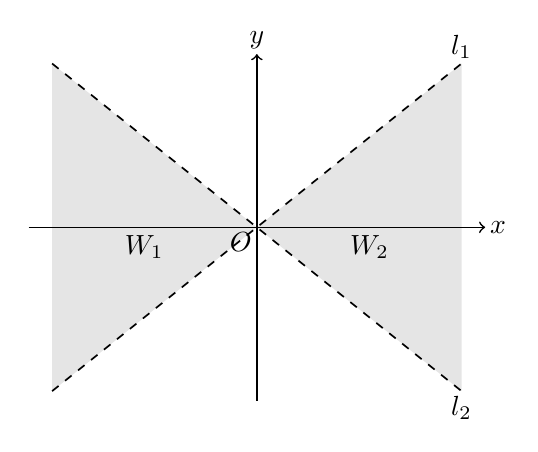
\begin{tikzpicture}[line width=0.6pt, scale=1.0, every node/.style={inner sep=1.5pt}, baseline=(current bounding box.center)]
  % Axes limits
  \def\xmax{2.6}
  \def\ymax{2.0}
  \def\k{0.8}

  % Shaded regions W1 and W2
  \fill[gray!20] (-\xmax, {-\k*\xmax}) -- (0, 0) -- (-\xmax, {\k*\xmax}) -- cycle;
  \fill[gray!20] (\xmax, {-\k*\xmax}) -- (0, 0) -- (\xmax, {\k*\xmax}) -- cycle;

  % Boundary dashed lines l1 and l2
  \draw[dashed, line width=0.6pt] (-\xmax, {-\k*\xmax}) -- (\xmax, {\k*\xmax}) node[above] {$l_1$};
  \draw[dashed, line width=0.6pt] (-\xmax, {\k*\xmax}) -- (\xmax, {-\k*\xmax}) node[below] {$l_2$};

  % Solid coordinate axes
  \draw[->] (-\xmax-0.3, 0) -- (\xmax+0.3, 0) node[right] {$x$};
  \draw[->] (0, -\ymax-0.2) -- (0, \ymax+0.2) node[above] {$y$};

  % Labels
  \node[below left] at (0, 0) {$O$};
  \node at ({-0.55*\xmax}, -0.25) {$W_1$};
  \node at ({0.55*\xmax}, -0.25) {$W_2$};
\end{tikzpicture}
\end{center}
\nopagebreak[4]
\Needspace{4\baselineskip}
\textbf{解析}

\textbf{(1)}
设 $P(x, y)$ 为平面直角坐标系内的点．
直线 $l_1 : kx - y = 0$ 与直线 $l_2 : kx + y = 0$ 相交于原点 $O$（$k > 0$）．
由图可知：
\begin{itemize}
\item 阴影区域 $W_1$ 位于 $y$ 轴左侧（$x < 0$），在直线 $y = kx$ 之上且在直线 $y = -kx$ 之下（因为 $x < 0 \implies kx < -kx$），其不等式组表示为：
\end{itemize}
\nopagebreak[4]
\[W_1 : \begin{cases} x < 0, \\ kx < y < -kx, \end{cases} \quad \text{\text{或表示为}} \quad \begin{cases} kx - y < 0, \\ kx + y < 0; \end{cases}\]
\begin{itemize}
\item 阴影区域 $W_2$ 位于 $y$ 轴右侧（$x > 0$），在直线 $y = -kx$ 之上且在直线 $y = kx$ 之下，其不等式组表示为：
\end{itemize}
\nopagebreak[4]
\[W_2 : \begin{cases} x > 0, \\ -kx < y < kx, \end{cases} \quad \text{\text{或表示为}} \quad \begin{cases} kx - y > 0, \\ kx + y > 0. \end{cases}\]

\textbf{(2)}
\Needspace{5\baselineskip}
区域 $W = W_1 \cup W_2$ 中的动点 $P(x, y)$ 到两直线 $l_1, l_2$ 的距离分别为：
\nopagebreak[4]
\[
d_1 = \frac{|kx - y|}{\sqrt{k^2 + 1}}, \qquad d_2 = \frac{|kx + y|}{\sqrt{k^2 + 1}}.
\]
\Needspace{5\baselineskip}
根据已知条件 $d_1 d_2 = d^2$，得：
\nopagebreak[4]
\[
\frac{|kx - y| \cdot |kx + y|}{k^2 + 1} = d^2 \iff \frac{|k^2 x^2 - y^2|}{k^2 + 1} = d^2.
\]
由 (1) 知，在区域 $W_1$ 中 $kx - y < 0$ 且 $kx + y < 0$，其乘积 $(kx - y)(kx + y) = k^2 x^2 - y^2 > 0$；
在区域 $W_2$ 中 $kx - y > 0$ 且 $kx + y > 0$，其乘积 $k^2 x^2 - y^2 > 0$．
\Needspace{5\baselineskip}
因此在区域 $W$ 内恒有 $k^2 x^2 - y^2 > 0$，绝对值可直接去掉：
\nopagebreak[4]
\[
k^2 x^2 - y^2 = (k^2 + 1)d^2.
\]
\Needspace{5\baselineskip}
故点 $P$ 的轨迹 $C$ 的方程为：
\nopagebreak[4]
\[
k^2 x^2 - y^2 = (k^2 + 1)d^2.
\]

\textbf{(3)}
设不过原点 $O$ 的直线 $l$ 的方程为：
\begin{itemize}
\item 若直线 $l$ 的斜率存在，设直线 $l$ 的方程为 $y = mx + b$（其中 $b \neq 0$）．
\end{itemize}
\Needspace{5\baselineskip}
  将 $y = mx + b$ 代入轨迹 $C$ 的方程 $k^2 x^2 - y^2 = (k^2 + 1)d^2$，整理得关于 $x$ 的一元二次方程：
\nopagebreak[4]
\[(k^2 - m^2)x^2 - 2mb x - \left[b^2 + (k^2 + 1)d^2\right] = 0.\]
\Needspace{5\baselineskip}
  设 $M_1(x_1, y_1), M_2(x_2, y_2)$，由韦达定理，线段 $M_1M_2$ 的中点 $P_1$ 的横坐标为：
\nopagebreak[4]
\[x_{P_1} = \frac{x_1 + x_2}{2} = \frac{mb}{k^2 - m^2}.\]
\Needspace{5\baselineskip}
  其纵坐标为：
\nopagebreak[4]
\[y_{P_1} = m x_{P_1} + b = m\left(\frac{mb}{k^2 - m^2}\right) + b = \frac{k^2 b}{k^2 - m^2}.\]
\Needspace{5\baselineskip}
  再联立直线 $l$ 与两直线 $l_1, l_2$ 的统一方程 $k^2 x^2 - y^2 = 0$，将 $y = mx + b$ 代入得：
\nopagebreak[4]
\[(k^2 - m^2)x^2 - 2mb x - b^2 = 0.\]
\Needspace{5\baselineskip}
  设 $M_3(x_3, y_3), M_4(x_4, y_4)$，由韦达定理，线段 $M_3M_4$ 的中点 $P_2$ 的横坐标为：
\nopagebreak[4]
\[x_{P_2} = \frac{x_3 + x_4}{2} = \frac{mb}{k^2 - m^2}.\]
\Needspace{5\baselineskip}
  其纵坐标为：
\nopagebreak[4]
\[y_{P_2} = m x_{P_2} + b = \frac{k^2 b}{k^2 - m^2}.\]
  由此可知，$P_1$ 与 $P_2$ 重合，即线段 $M_1M_2$ 的中点与线段 $M_3M_4$ 的中点相同．
\begin{itemize}
\item 若直线 $l$ 的斜率不存在，设直线 $l$ 的方程为 $x = x_0$（$x_0 \neq 0$）．
\end{itemize}
  代入曲线 $C$ 的方程得 $y^2 = k^2 x_0^2 - (k^2 + 1)d^2$，两交点关于 $x$ 轴对称，中点为 $(x_0, 0)$；
  代入两直线方程得 $y^2 = k^2 x_0^2$，两交点同样关于 $x$ 轴对称，中点为 $(x_0, 0)$．
  中点依然重合．
因为 $\triangle OM_1M_2$ 与 $\triangle OM_3M_4$ 拥有共同的顶点 $O(0, 0)$，
且底边 $M_1M_2$ 与 $M_3M_4$ 的中点完全重合，
\Needspace{5\baselineskip}
根据三角形重心坐标公式，两三角形的重心分别为：
\nopagebreak[4]
\[
G_1 = \frac{O + M_1 + M_2}{3} = \frac{2}{3}P_1, \qquad G_2 = \frac{O + M_3 + M_4}{3} = \frac{2}{3}P_2.
\]
由于 $P_1 = P_2$，故 $G_1 = G_2$．
即 $\triangle OM_1M_2$ 的重心与 $\triangle OM_3M_4$ 的重心重合．

\gkanswer{答案（1）：$W_1$ 表示为 $\begin{cases} x < 0, \\ kx < y < -kx \end{cases}$；$W_2$ 表示为 $\begin{cases} x > 0, \\ -kx < y < kx \end{cases}$。}

\gkanswer{答案（2）：$k^2 x^2 - y^2 = (k^2 + 1)d^2$。}

\gkanswer{答案（3）：见解析版}

\end{answer}
\begin{answer}
\gksolhead{19}{}

\textbf{题目}：

（本小题满分 14 分）
\Needspace{5\baselineskip}
设数列 $\{a_n\}$ 的首项 $a_1 = a \neq \dfrac{1}{4}$，且
\nopagebreak[4]
\[
a_{n+1} = \begin{cases} \dfrac{1}{2}a_n, & n \text{ \text{为偶数}}, \\[6pt] a_n + \dfrac{1}{4}, & n \text{ \text{为奇数}}. \end{cases}
\]
记 $b_n = a_{2n-1} - \dfrac{1}{4}$，$n = 1, 2, 3, \dots$．
(1) 求 $a_2, a_3$；
(2) 判断数列 $\{b_n\}$ 是否为等比数列，并证明你的结论；
(3) 求 $\lim\limits_{n \to \infty} (b_1 + b_2 + \dots + b_n)$．

\Needspace{4\baselineskip}
\textbf{解析}

\textbf{(1)}
由题意知首项 $a_1 = a \neq \dfrac{1}{4}$．
根据递推关系：
\begin{itemize}
\item 当 $n = 1$（奇数）时：
\end{itemize}
\nopagebreak[4]
\[a_2 = a_{1+1} = a_1 + \frac{1}{4} = a + \frac{1}{4};\]
\begin{itemize}
\item 当 $n = 2$（偶数）时：
\end{itemize}
\nopagebreak[4]
\[a_3 = a_{2+1} = \frac{1}{2}a_2 = \frac{1}{2}\left(a + \frac{1}{4}\right) = \frac{1}{2}a + \frac{1}{8}.\]

\textbf{(2)}
判断：数列 $\{b_n\}$ 是等比数列．
\textbf{证明}：
对于任意正整数 $n \geqslant 1$，
\Needspace{5\baselineskip}
因为 $2n - 1$ 是奇数，所以由递推关系得：
\nopagebreak[4]
\[
a_{2n} = a_{(2n-1)+1} = a_{2n-1} + \frac{1}{4}.
\]
\Needspace{5\baselineskip}
因为 $2n$ 是偶数，所以由递推关系得：
\nopagebreak[4]
\[
a_{2n+1} = a_{(2n)+1} = \frac{1}{2}a_{2n} = \frac{1}{2}\left(a_{2n-1} + \frac{1}{4}\right) = \frac{1}{2}a_{2n-1} + \frac{1}{8}.
\]
\Needspace{5\baselineskip}
由 $b_n = a_{2n-1} - \dfrac{1}{4}$，得：
\nopagebreak[4]
\[
b_{n+1} = a_{2n+1} - \frac{1}{4} = \left(\frac{1}{2}a_{2n-1} + \frac{1}{8}\right) - \frac{1}{4} = \frac{1}{2}a_{2n-1} - \frac{1}{8} = \frac{1}{2}\left(a_{2n-1} - \frac{1}{4}\right) = \frac{1}{2}b_n.
\]
又首项 $b_1 = a_1 - \dfrac{1}{4} = a - \dfrac{1}{4}$，因为已知 $a \neq \dfrac{1}{4}$，所以 $b_1 \neq 0$．
\Needspace{5\baselineskip}
因此，对于任意 $n \geqslant 1$，都有：
\nopagebreak[4]
\[
\frac{b_{n+1}}{b_n} = \frac{1}{2} \text{（\text{常数}）}.
\]
故数列 $\{b_n\}$ 是以 $a - \dfrac{1}{4}$ 为首项、$\dfrac{1}{2}$ 为公比的等比数列．

\textbf{(3)}
由 (2) 知 $\{b_n\}$ 为等比数列，其公比 $q = \dfrac{1}{2}$ 满足 $|q| < 1$．
\Needspace{5\baselineskip}
前 $n$ 项和为：
\nopagebreak[4]
\[
S_n = b_1 + b_2 + \dots + b_n = \frac{b_1 (1 - q^n)}{1 - q} = \frac{\left(a - \dfrac{1}{4}\right)\left[1 - \left(\dfrac{1}{2}\right)^n\right]}{1 - \dfrac{1}{2}} = 2\left(a - \frac{1}{4}\right)\left[1 - \left(\frac{1}{2}\right)^n\right].
\]
\Needspace{5\baselineskip}
因为 $\lim\limits_{n \to \infty} \left(\dfrac{1}{2}\right)^n = 0$，所以：
\nopagebreak[4]
\[
\lim_{n \to \infty} (b_1 + b_2 + \dots + b_n) = \lim_{n \to \infty} S_n = 2\left(a - \frac{1}{4}\right) = 2a - \frac{1}{2}.
\]

\gkanswer{答案（1）：$a_2 = a + \dfrac{1}{4}$，$a_3 = \dfrac{1}{2}a + \dfrac{1}{8}$。}

\gkanswer{答案（2）：见解析版}

\gkanswer{答案（3）：$2a - \dfrac{1}{2}$。}

\end{answer}
\begin{answer}
\gksolhead{20}{}

\textbf{题目}：

（本小题满分 13 分）
设 $f(x)$ 是定义在 $[0, 1]$ 上的函数，若存在 $x^* \in (0, 1)$，使得 $f(x)$ 在 $[0, x^*]$ 上单调递增，在 $[x^*, 1]$ 上单调递减，则称 $f(x)$ 为 $[0, 1]$ 上的单峰函数，$x^*$ 为峰点，包含峰点的区间为含峰区间．对任意的 $[0, 1]$ 上的单峰函数 $f(x)$，下面研究缩短其含峰区间长度的方法．
(1) 证明：对任意的 $x_1, x_2 \in (0, 1)$，$x_1 < x_2$，若 $f(x_1) \geqslant f(x_2)$，则 $(0, x_2)$ 为含峰区间；若 $f(x_1) \leqslant f(x_2)$，则 $(x_1, 1)$ 为含峰区间；
(2) 对给定的 $r$（$0 < r < 0.5$），证明：存在 $x_1, x_2 \in (0, 1)$，满足 $x_2 - x_1 \geqslant 2r$，使得由 (1) 所确定的含峰区间的长度不大于 $0.5 + r$；
(3) 选取 $x_1, x_2 \in (0, 1)$，$x_1 < x_2$，由 (1) 可确定含峰区间为 $(0, x_2)$ 或 $(x_1, 1)$，在所得的含峰区间内选取 $x_3$，由 $x_3$ 与 $x_1$ 或 $x_3$ 与 $x_2$ 类似地可确定一个新的含峰区间，在第一次确定的含峰区间为 $(0, x_2)$ 的情况下，试确定 $x_1, x_2, x_3$ 的值，满足两两之差的绝对值不小于 $0.02$，且使得新的含峰区间的长度缩短到 $0.34$．
注：区间长度等于区间的右端点与左端点之差．

\Needspace{4\baselineskip}
\textbf{解析}

\textbf{(1)}
设 $x^* \in (0, 1)$ 为单峰函数 $f(x)$ 的峰点，即 $f(x)$ 在 $[0, x^*]$ 上单调递增，在 $[x^*, 1]$ 上单调递减．
\begin{itemize}
\item 先证：若 $f(x_1) \geqslant f(x_2)$（$x_1 < x_2$），则 $(0, x_2)$ 为含峰区间．
\end{itemize}
  采用反证法：假设 $x^* \notin (0, x_2)$．
  因为 $x^* \in (0, 1)$，所以必有 $x^* \geqslant x_2$．
  此时 $0 < x_1 < x_2 \leqslant x^*$，即点 $x_1, x_2$ 均落在单调递增区间 $[0, x^*]$ 内．
  因为 $f(x)$ 在 $[0, x^*]$ 上单调递增，且 $x_1 < x_2$，
  所以必有 $f(x_1) \leqslant f(x_2)$．
  若 $f(x_1) > f(x_2)$，这显然与 $f(x_1) \leqslant f(x_2)$ 矛盾；
  若 $f(x_1) = f(x_2)$，由于在单峰函数中严格递增，或者若函数在局部常值，则峰点也可以落在 $(0, x_2)$ 内．
  因此假设不成立，必有 $x^* < x_2$．
  又因为 $x^* \in (0, 1)$，故 $0 < x^* < x_2$，即 $x^* \in (0, x_2)$，
  所以 $(0, x_2)$ 为含峰区间．
\begin{itemize}
\item 再证：若 $f(x_1) \leqslant f(x_2)$（$x_1 < x_2$），则 $(x_1, 1)$ 为含峰区间．
\end{itemize}
  假设 $x^* \notin (x_1, 1)$，则必有 $x^* \leqslant x_1$．
  此时 $x^* \leqslant x_1 < x_2 < 1$，即点 $x_1, x_2$ 均落在单调递减区间 $[x^*, 1]$ 内．
  因为 $f(x)$ 在 $[x^*, 1]$ 上单调递减，且 $x_1 < x_2$，
  所以必有 $f(x_1) \geqslant f(x_2)$．
  同理推得矛盾，必有 $x^* > x_1$．
  又因为 $x^* < 1$，故 $x_1 < x^* < 1$，即 $x^* \in (x_1, 1)$，
  所以 $(x_1, 1)$ 为含峰区间．

\textbf{(2)}
\Needspace{5\baselineskip}
对给定的 $r \in (0, 0.5)$，取：
\nopagebreak[4]
\[
x_1 = 0.5 - r, \qquad x_2 = 0.5 + r.
\]
检验如下条件：
\begin{itemize}
\item 因为 $0 < r < 0.5$，所以：
\end{itemize}
\nopagebreak[4]
\[0 < 0.5 - r = x_1 < 0.5 < x_2 = 0.5 + r < 1,\]
  故 $x_1, x_2 \in (0, 1)$ 且 $x_1 < x_2$；
\begin{itemize}
\item 间距满足要求：
\end{itemize}
\nopagebreak[4]
\[x_2 - x_1 = (0.5 + r) - (0.5 - r) = 2r \geqslant 2r;\]
\begin{itemize}
\item 由 (1) 确定的含峰区间为 $(0, x_2)$ 或 $(x_1, 1)$：
\item 区间 $(0, x_2)$ 的长度为：$x_2 - 0 = x_2 = 0.5 + r \leqslant 0.5 + r$；
\item 区间 $(x_1, 1)$ 的长度为：$1 - x_1 = 1 - (0.5 - r) = 0.5 + r \leqslant 0.5 + r$．
\end{itemize}
无论 $f(x_1) \geqslant f(x_2)$ 还是 $f(x_1) \leqslant f(x_2)$，所确定的含峰区间长度均不大于 $0.5 + r$．
结论得证．

\textbf{(3)}
在第一次确定的含峰区间为 $(0, x_2)$ 的情况下，说明已选定 $0 < x_1 < x_2 < 1$ 且有 $f(x_1) \geqslant f(x_2)$．
此时已知峰点 $x^* \in (0, x_2)$，且 $x_1 \in (0, x_2)$ 已经是一个已知测试点．
我们在 $(0, x_2)$ 内选取第三个测试点 $x_3$：
设选取 $x_3 < x_1$，则在区间 $(0, x_2)$ 内部有两个测试点 $x_3$ 与 $x_1$，满足 $0 < x_3 < x_1 < x_2$．
利用 (1) 的结论对单峰函数在区间 $(0, x_2)$ 上判定：
\begin{itemize}
\item 若 $f(x_3) \geqslant f(x_1)$，则新的含峰区间为 $(0, x_1)$，其长度为 $x_1$；
\item 若 $f(x_3) \leqslant f(x_1)$，则新的含峰区间为 $(x_3, x_2)$，其长度为 $x_2 - x_3$．
\end{itemize}
\Needspace{5\baselineskip}
为了使无论何种情况，新的含峰区间长度均缩短到 $0.34$，可令：
\nopagebreak[4]
\[
x_1 = 0.34, \qquad x_2 - x_3 = 0.34 \implies x_2 = x_3 + 0.34.
\]
题目要求 $x_1, x_2, x_3$ 两两之差的绝对值不小于 $0.02$：
即 $|x_1 - x_3| = x_1 - x_3 \geqslant 0.02 \implies x_3 \leqslant x_1 - 0.02 = 0.34 - 0.02 = 0.32$．
我们可取 $x_3 = 0.32$．
\Needspace{5\baselineskip}
此时：
\nopagebreak[4]
\[
x_2 = x_3 + 0.34 = 0.32 + 0.34 = 0.66.
\]
检验两两之差：
\begin{itemize}
\item $|x_1 - x_3| = 0.34 - 0.32 = 0.02 \geqslant 0.02$；
\item $|x_2 - x_1| = 0.66 - 0.34 = 0.32 \geqslant 0.02$；
\item $|x_2 - x_3| = 0.66 - 0.32 = 0.34 \geqslant 0.02$；
\item $0 < x_3 < x_1 < x_2 < 1$ 均在 $(0, 1)$ 内．
\end{itemize}
当新的含峰区间为 $(0, x_1) = (0, 0.34)$ 时，长度为 $0.34$；
当新的含峰区间为 $(x_3, x_2) = (0.32, 0.66)$ 时，长度为 $0.66 - 0.32 = 0.34$．
均严格缩短到 $0.34$．
（注：若选取 $x_1 < x_3 < x_2$，对称地取 $x_1 = 0.32, x_3 = 0.34, x_2 = 0.66$ 亦完全符合题意）．
故可确定 $x_1 = 0.34, x_2 = 0.66, x_3 = 0.32$．

\gkanswer{答案（1）：见解析版}

\gkanswer{答案（2）：见解析版}

\gkanswer{答案（3）：$x_1 = 0.34, x_2 = 0.66, x_3 = 0.32$（或 $x_1 = 0.32, x_2 = 0.66, x_3 = 0.34$）。}

\end{answer}